\documentclass[11pt]{article}

\usepackage[letterpaper,landscape,margin=0.45in]{geometry}
\usepackage[T1]{fontenc}
\usepackage{lmodern}
\usepackage{amsmath}
\usepackage{tikz}
\usetikzlibrary{
  arrows.meta,
  calc,
  fit,
  positioning,
  backgrounds,
  decorations.pathreplacing,
  shapes.geometric,
  shapes.misc,
  shapes.symbols
}

\pagestyle{empty}
\setlength{\parindent}{0pt}

\definecolor{datasetFill}{RGB}{221,236,214}
\definecolor{datasetStroke}{RGB}{127,167,108}
\definecolor{processFill}{RGB}{251,241,207}
\definecolor{processStroke}{RGB}{217,176,80}
\definecolor{accentFill}{RGB}{252,235,213}
\definecolor{accentStroke}{RGB}{220,148,37}
\definecolor{blueFill}{RGB}{219,232,250}
\definecolor{blueStroke}{RGB}{98,138,197}
\definecolor{tealFill}{RGB}{215,235,231}
\definecolor{tealStroke}{RGB}{71,144,129}
\definecolor{amberFill}{RGB}{244,228,194}
\definecolor{amberStroke}{RGB}{190,144,45}
\definecolor{warnFill}{RGB}{248,224,224}
\definecolor{warnStroke}{RGB}{181,77,77}
\colorlet{ink}{black!82}

\tikzset{
  >={Latex[length=3mm,width=2mm]},
  arrow/.style={-{Latex[length=3mm,width=2mm]}, draw=ink, line width=0.95pt},
  connector/.style={draw=ink, line width=0.95pt},
  process/.style={
    draw=processStroke,
    fill=processFill,
    rounded corners=7pt,
    line width=0.95pt,
    minimum height=1.35cm,
    text width=3.6cm,
    inner sep=6pt,
    font=\sffamily\small
  },
  accentbox/.style={
    draw=accentStroke,
    fill=accentFill,
    rounded corners=8pt,
    line width=1.0pt,
    minimum height=1.35cm,
    text width=3.8cm,
    inner sep=7pt,
    font=\sffamily\small
  },
  bluebox/.style={
    draw=blueStroke,
    fill=blueFill,
    rounded corners=8pt,
    line width=0.95pt,
    minimum height=1.35cm,
    text width=3.8cm,
    inner sep=7pt,
    font=\sffamily\small
  },
  tealbox/.style={
    draw=tealStroke,
    fill=tealFill,
    rounded corners=8pt,
    line width=0.95pt,
    minimum height=1.35cm,
    text width=3.8cm,
    inner sep=7pt,
    font=\sffamily\small
  },
  amberbox/.style={
    draw=amberStroke,
    fill=amberFill,
    rounded corners=8pt,
    line width=0.95pt,
    minimum height=1.35cm,
    text width=3.8cm,
    inner sep=7pt,
    font=\sffamily\small
  },
  warnbox/.style={
    draw=warnStroke,
    fill=warnFill,
    rounded corners=8pt,
    line width=0.95pt,
    minimum height=1.35cm,
    text width=3.8cm,
    inner sep=7pt,
    font=\sffamily\small
  },
  plainbox/.style={
    draw=black!32,
    fill=white,
    rounded corners=5pt,
    line width=0.8pt,
    inner sep=5pt,
    align=center,
    font=\sffamily\small
  },
  note/.style={
    draw=black!26,
    fill=white,
    rectangle,
    rounded corners=2pt,
    inner sep=4pt,
    font=\sffamily\footnotesize,
    text=ink
  },
  databox/.style={
    cylinder,
    draw=datasetStroke,
    fill=datasetFill,
    line width=1.0pt,
    shape aspect=0.35,
    minimum width=2.25cm,
    minimum height=3.0cm,
    inner sep=4pt,
    align=center,
    font=\sffamily\small
  },
  cloudbox/.style={
    cloud,
    cloud puffs=12,
    cloud ignores aspect,
    draw=blueStroke,
    fill=blueFill,
    line width=0.95pt,
    minimum width=4.1cm,
    minimum height=2.25cm,
    align=center,
    font=\sffamily\small
  },
  outline/.style={draw=black!20, rounded corners=10pt, line width=0.7pt},
  tiny label/.style={font=\sffamily\scriptsize, text=black!65}
}

\tikzset{
  pics/hexagon/.style={
    code={
      \coordinate (-A) at (90:0.75);
      \coordinate (-B) at (30:0.75);
      \coordinate (-C) at (-30:0.75);
      \coordinate (-D) at (-90:0.75);
      \coordinate (-E) at (-150:0.75);
      \coordinate (-F) at (150:0.75);
      \draw[draw=ink, fill=processFill!92, line width=0.9pt]
        (-A) -- (-B) -- (-C) -- (-D) -- (-E) -- (-F) -- cycle;
      \foreach \p in {A,B,C,D,E,F}{
        \fill[ink] (-\p) circle (1.1pt);
      }
    }
  },
  pics/irregularpoly/.style={
    code={
      \coordinate (-A) at (95:0.78);
      \coordinate (-B) at (28:0.63);
      \coordinate (-C) at (-18:0.84);
      \coordinate (-D) at (-85:0.68);
      \coordinate (-E) at (-158:0.87);
      \coordinate (-F) at (160:0.58);
      \draw[draw=ink, fill=blueFill!78, line width=0.9pt]
        (-A) -- (-B) -- (-C) -- (-D) -- (-E) -- (-F) -- cycle;
      \foreach \p in {A,B,C,D,E,F}{
        \fill[ink] (-\p) circle (1.1pt);
      }
    }
  }
}

\newcommand{\PageTitle}[1]{%
  \node[font=\sffamily\bfseries\Large, text=ink] at (13.2,18.45) {#1};
}

\newcommand{\PageSubtitle}[1]{%
  \node[font=\sffamily\small, text=black!60] at (13.2,17.72) {#1};
}

\begin{document}

% --------------------------------------------------------------------------
% Figure 1
% --------------------------------------------------------------------------
\begin{center}
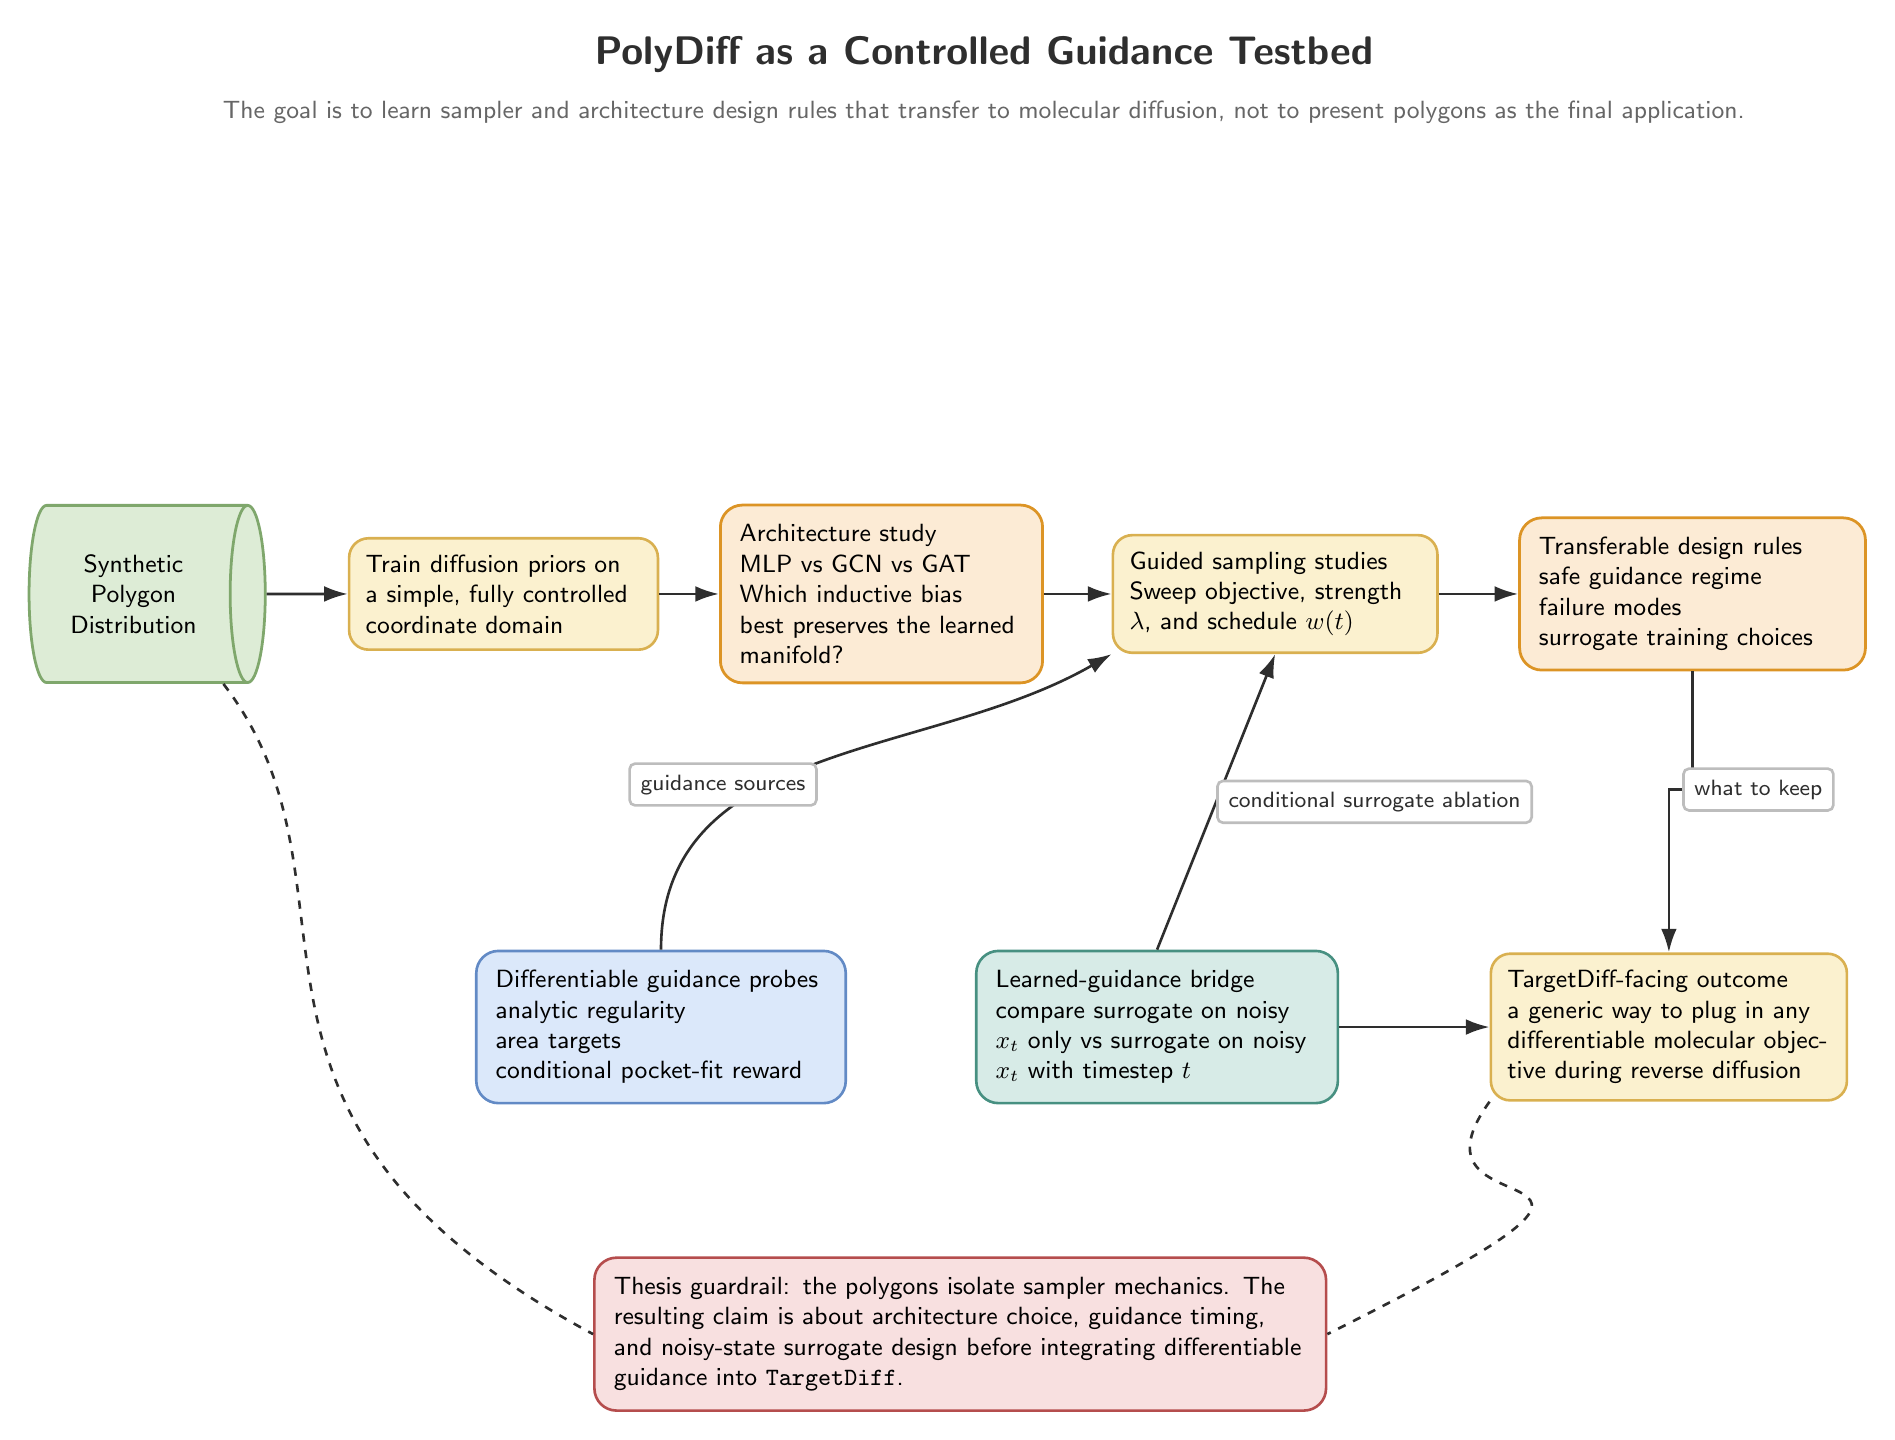
\begin{tikzpicture}[x=1cm,y=1cm]
  \PageTitle{PolyDiff as a Controlled Guidance Testbed}
  \PageSubtitle{The goal is to learn sampler and architecture design rules that transfer to molecular diffusion, not to present polygons as the final application.}

  \node[databox] (polydata) at (2.4,11.6) {Synthetic\\Polygon\\Distribution};
  \node[process, text width=3.5cm] (priortrain) at (7.1,11.6) {Train diffusion priors on a simple, fully controlled coordinate domain};
  \node[accentbox, text width=3.6cm] (archstudy) at (11.9,11.6) {Architecture study\\MLP vs GCN vs GAT\\Which inductive bias best preserves the learned manifold?};
  \node[process, text width=3.7cm] (guidestudy) at (16.9,11.6) {Guided sampling studies\\Sweep objective, strength $\lambda$, and schedule $w(t)$};
  \node[accentbox, text width=3.9cm] (rules) at (22.2,11.6) {Transferable design rules\\safe guidance regime\\failure modes\\surrogate training choices};

  \node[bluebox, text width=4.2cm] (objectives) at (9.1,6.1) {Differentiable guidance probes\\analytic regularity\\area targets\\conditional pocket-fit reward};
  \node[tealbox, text width=4.1cm] (surrogate) at (15.4,6.1) {Learned-guidance bridge\\compare surrogate on noisy $x_t$ only vs surrogate on noisy $x_t$ with timestep $t$};
  \node[process, text width=4.1cm] (targetdiff) at (21.9,6.1) {TargetDiff-facing outcome\\a generic way to plug in any differentiable molecular objective during reverse diffusion};

  \draw[arrow] (polydata.east) -- (priortrain.west);
  \draw[arrow] (priortrain.east) -- (archstudy.west);
  \draw[arrow] (archstudy.east) -- (guidestudy.west);
  \draw[arrow] (guidestudy.east) -- (rules.west);

  \draw[arrow] (objectives.north) to[out=90,in=-150] node[note, midway, below left] {guidance sources} (guidestudy.south west);
  \draw[arrow] (surrogate.north) -- node[note, right] {conditional surrogate ablation} (guidestudy.south);
  \draw[arrow] (surrogate.east) -- (targetdiff.west);
  \draw[arrow] (rules.south) -- ++(0,-1.5) -| node[note, pos=0.22, right] {what to keep} (targetdiff.north);

  \node[warnbox, text width=8.8cm, minimum height=1.5cm] (guardrail) at (12.9,2.2) {Thesis guardrail: the polygons isolate sampler mechanics. The resulting claim is about architecture choice, guidance timing, and noisy-state surrogate design before integrating differentiable guidance into \texttt{TargetDiff}.};

  \draw[connector, dashed] (polydata.south east) .. controls +(2.0,-2.6) and +(-5.2,2.8) .. (guardrail.west);
  \draw[connector, dashed] (targetdiff.south west) .. controls +(-1.3,-1.8) and +(5.2,2.6) .. (guardrail.east);
\end{tikzpicture}
\end{center}
\newpage

% --------------------------------------------------------------------------
% Figure 2
% --------------------------------------------------------------------------
\begin{center}
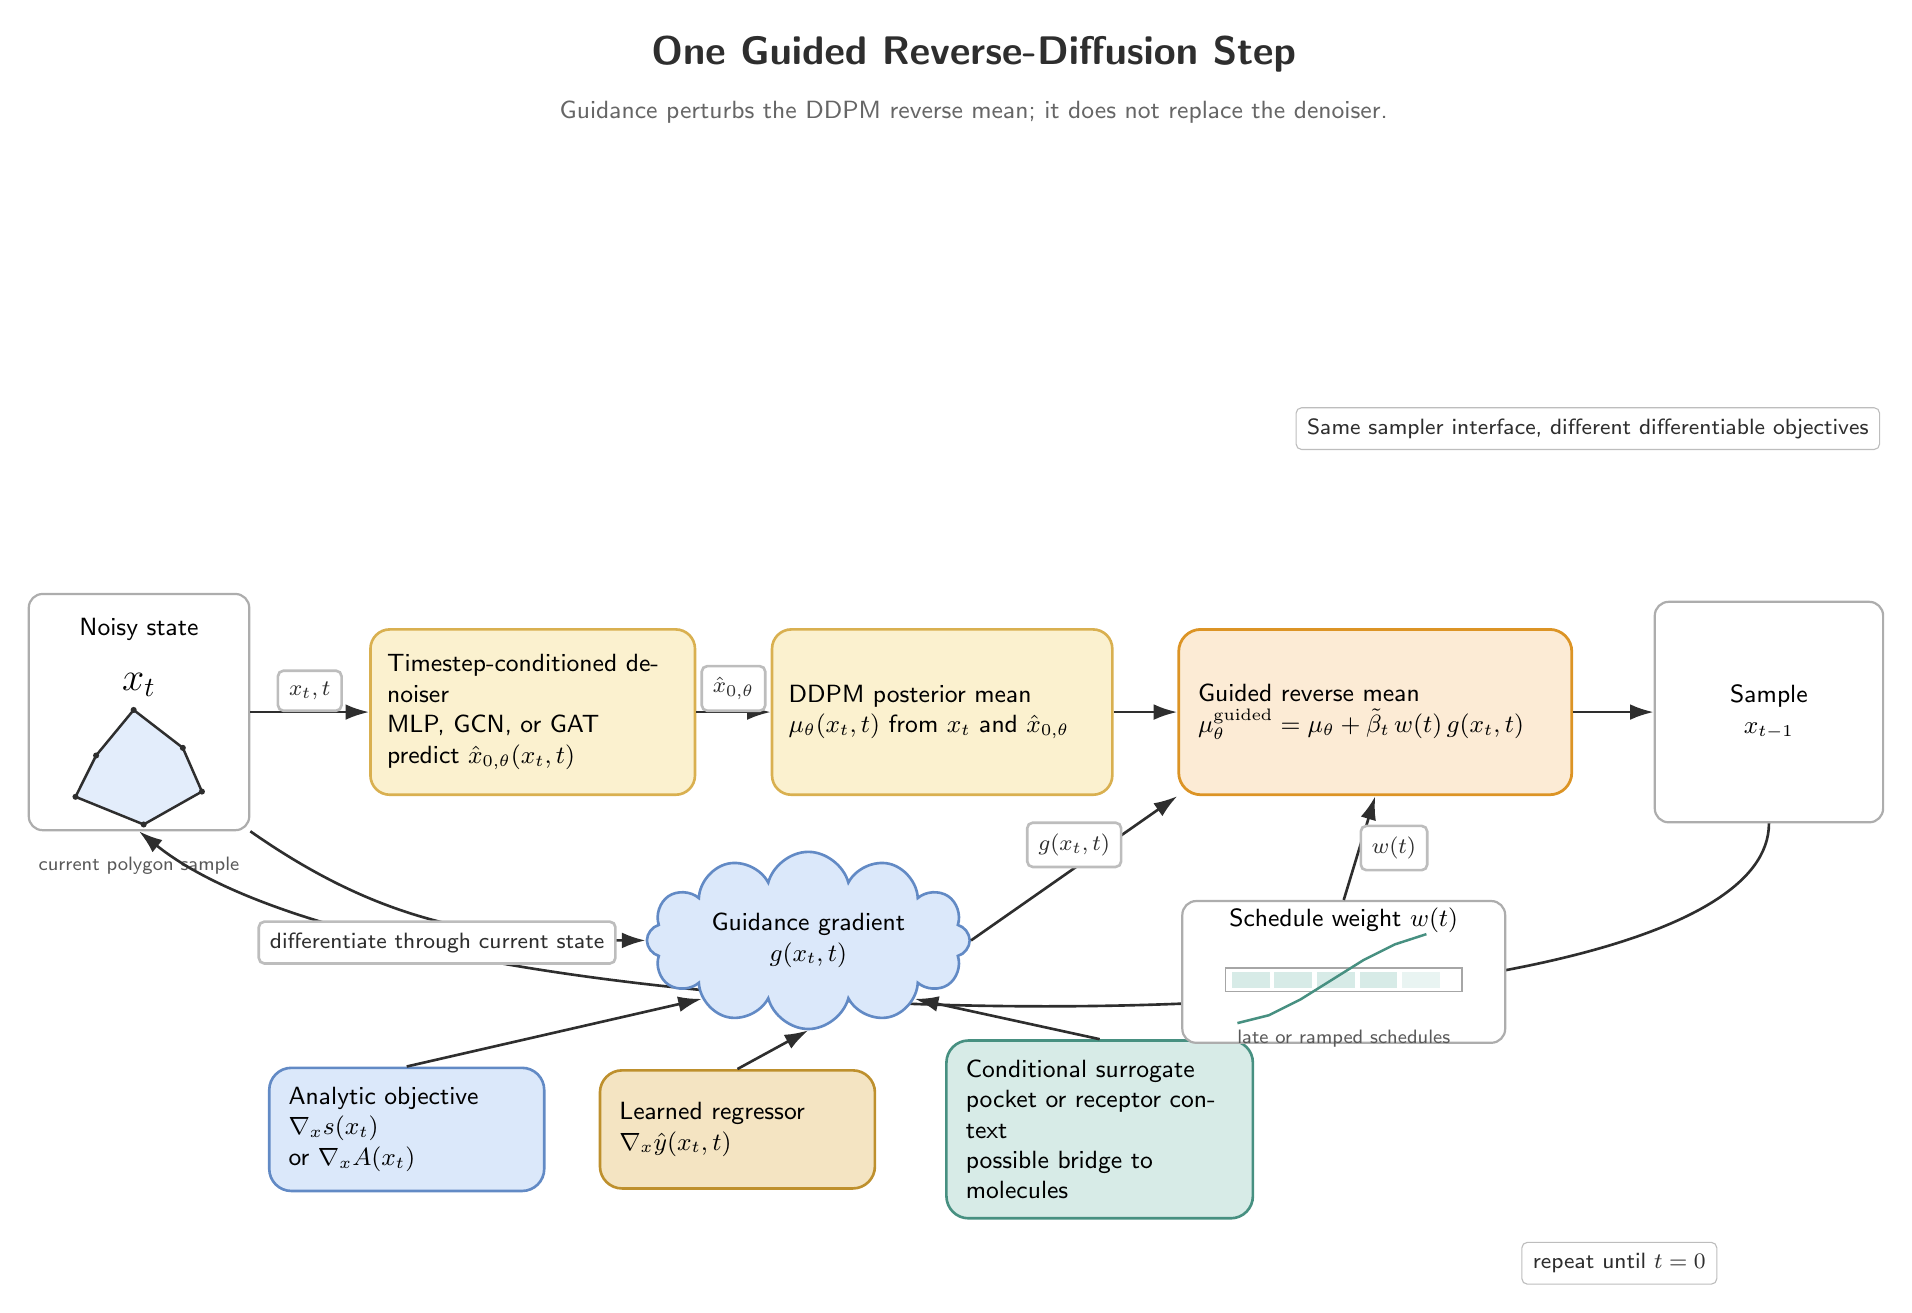
\begin{tikzpicture}[x=1cm,y=1cm]
  \PageTitle{One Guided Reverse-Diffusion Step}
  \PageSubtitle{Guidance perturbs the DDPM reverse mean; it does not replace the denoiser.}

  \node[plainbox, minimum width=2.8cm, minimum height=3.0cm] (xtbox) at (2.6,10.1) {};
  \node[font=\sffamily\small] at (2.6,11.15) {Noisy state};
  \node[font=\sffamily\Large] at (2.6,10.45) {$x_t$};
  \pic at (2.6,9.35) {irregularpoly};
  \node[tiny label] at (2.6,8.15) {current polygon sample};

  \node[process, text width=3.7cm, minimum height=2.1cm] (denoiser) at (7.6,10.1) {Timestep-conditioned denoiser\\MLP, GCN, or GAT\\predict $\hat{x}_{0,\theta}(x_t,t)$};
  \node[process, text width=3.9cm, minimum height=2.1cm] (posterior) at (12.8,10.1) {DDPM posterior mean\\$\mu_\theta(x_t,t)$ from $x_t$ and $\hat{x}_{0,\theta}$};
  \node[accentbox, text width=4.5cm, minimum height=2.1cm] (guidedmean) at (18.3,10.1) {Guided reverse mean\\$\mu_\theta^{\mathrm{guided}} = \mu_\theta + \tilde{\beta}_t\,w(t)\,g(x_t,t)$};
  \node[plainbox, minimum width=2.9cm, minimum height=2.8cm] (xtminus) at (23.3,10.1) {Sample\\$x_{t-1}$};

  \draw[arrow] (xtbox.east) -- node[note, above] {$x_t,t$} (denoiser.west);
  \draw[arrow] (denoiser.east) -- node[note, above] {$\hat{x}_{0,\theta}$} (posterior.west);
  \draw[arrow] (posterior.east) -- (guidedmean.west);
  \draw[arrow] (guidedmean.east) -- (xtminus.west);
  \draw[arrow] (xtminus.south) .. controls +(0,-3.1) and +(3.6,-2.9) .. (xtbox.south);
  \node[note] at (21.4,3.1) {repeat until $t=0$};

  \node[bluebox, text width=3.0cm, minimum height=1.5cm] (analytic) at (6.0,4.8) {Analytic objective\\$\nabla_x s(x_t)$\\or $\nabla_x A(x_t)$};
  \node[amberbox, text width=3.0cm, minimum height=1.5cm] (learned) at (10.2,4.8) {Learned regressor\\$\nabla_x \hat{y}(x_t,t)$};
  \node[tealbox, text width=3.4cm, minimum height=1.5cm] (conditional) at (14.8,4.8) {Conditional surrogate\\pocket or receptor context\\possible bridge to molecules};
  \node[cloudbox] (grad) at (11.1,7.2) {Guidance gradient\\$g(x_t,t)$};
  \node[plainbox, minimum width=4.1cm, minimum height=1.8cm] (schedule) at (17.9,6.8) {};
  \node[font=\sffamily\small] at (17.9,7.45) {Schedule weight $w(t)$};
  \draw[black!35, line width=0.5pt] (16.4,6.55) rectangle (19.4,6.85);
  \fill[tealFill] (16.48,6.60) rectangle (16.96,6.80);
  \fill[tealFill] (17.02,6.60) rectangle (17.50,6.80);
  \fill[tealFill] (17.56,6.60) rectangle (18.04,6.80);
  \fill[tealFill] (18.10,6.60) rectangle (18.58,6.80);
  \fill[tealFill!55!white] (18.64,6.60) rectangle (19.12,6.80);
  \draw[connector, line width=0.9pt, tealStroke] (16.55,6.15) -- (16.95,6.25) -- (17.35,6.45) -- (17.75,6.70) -- (18.15,6.95) -- (18.55,7.15) -- (18.95,7.28);
  \node[tiny label] at (17.9,5.95) {late or ramped schedules};

  \draw[arrow] (analytic.north) -- (grad.south west);
  \draw[arrow] (learned.north) -- (grad.south);
  \draw[arrow] (conditional.north) -- (grad.south east);
  \draw[arrow] (grad.east) -- node[note, above] {$g(x_t,t)$} (guidedmean.south west);
  \draw[arrow] (schedule.north) -- node[note, right] {$w(t)$} (guidedmean.south);
  \draw[arrow] (xtbox.south east) to[out=-35,in=180] node[note, below] {differentiate through current state} (grad.west);

  \node[note] at (21.0,13.7) {Same sampler interface, different differentiable objectives};
\end{tikzpicture}
\end{center}
\newpage

% --------------------------------------------------------------------------
% Figure 3
% --------------------------------------------------------------------------
\begin{center}
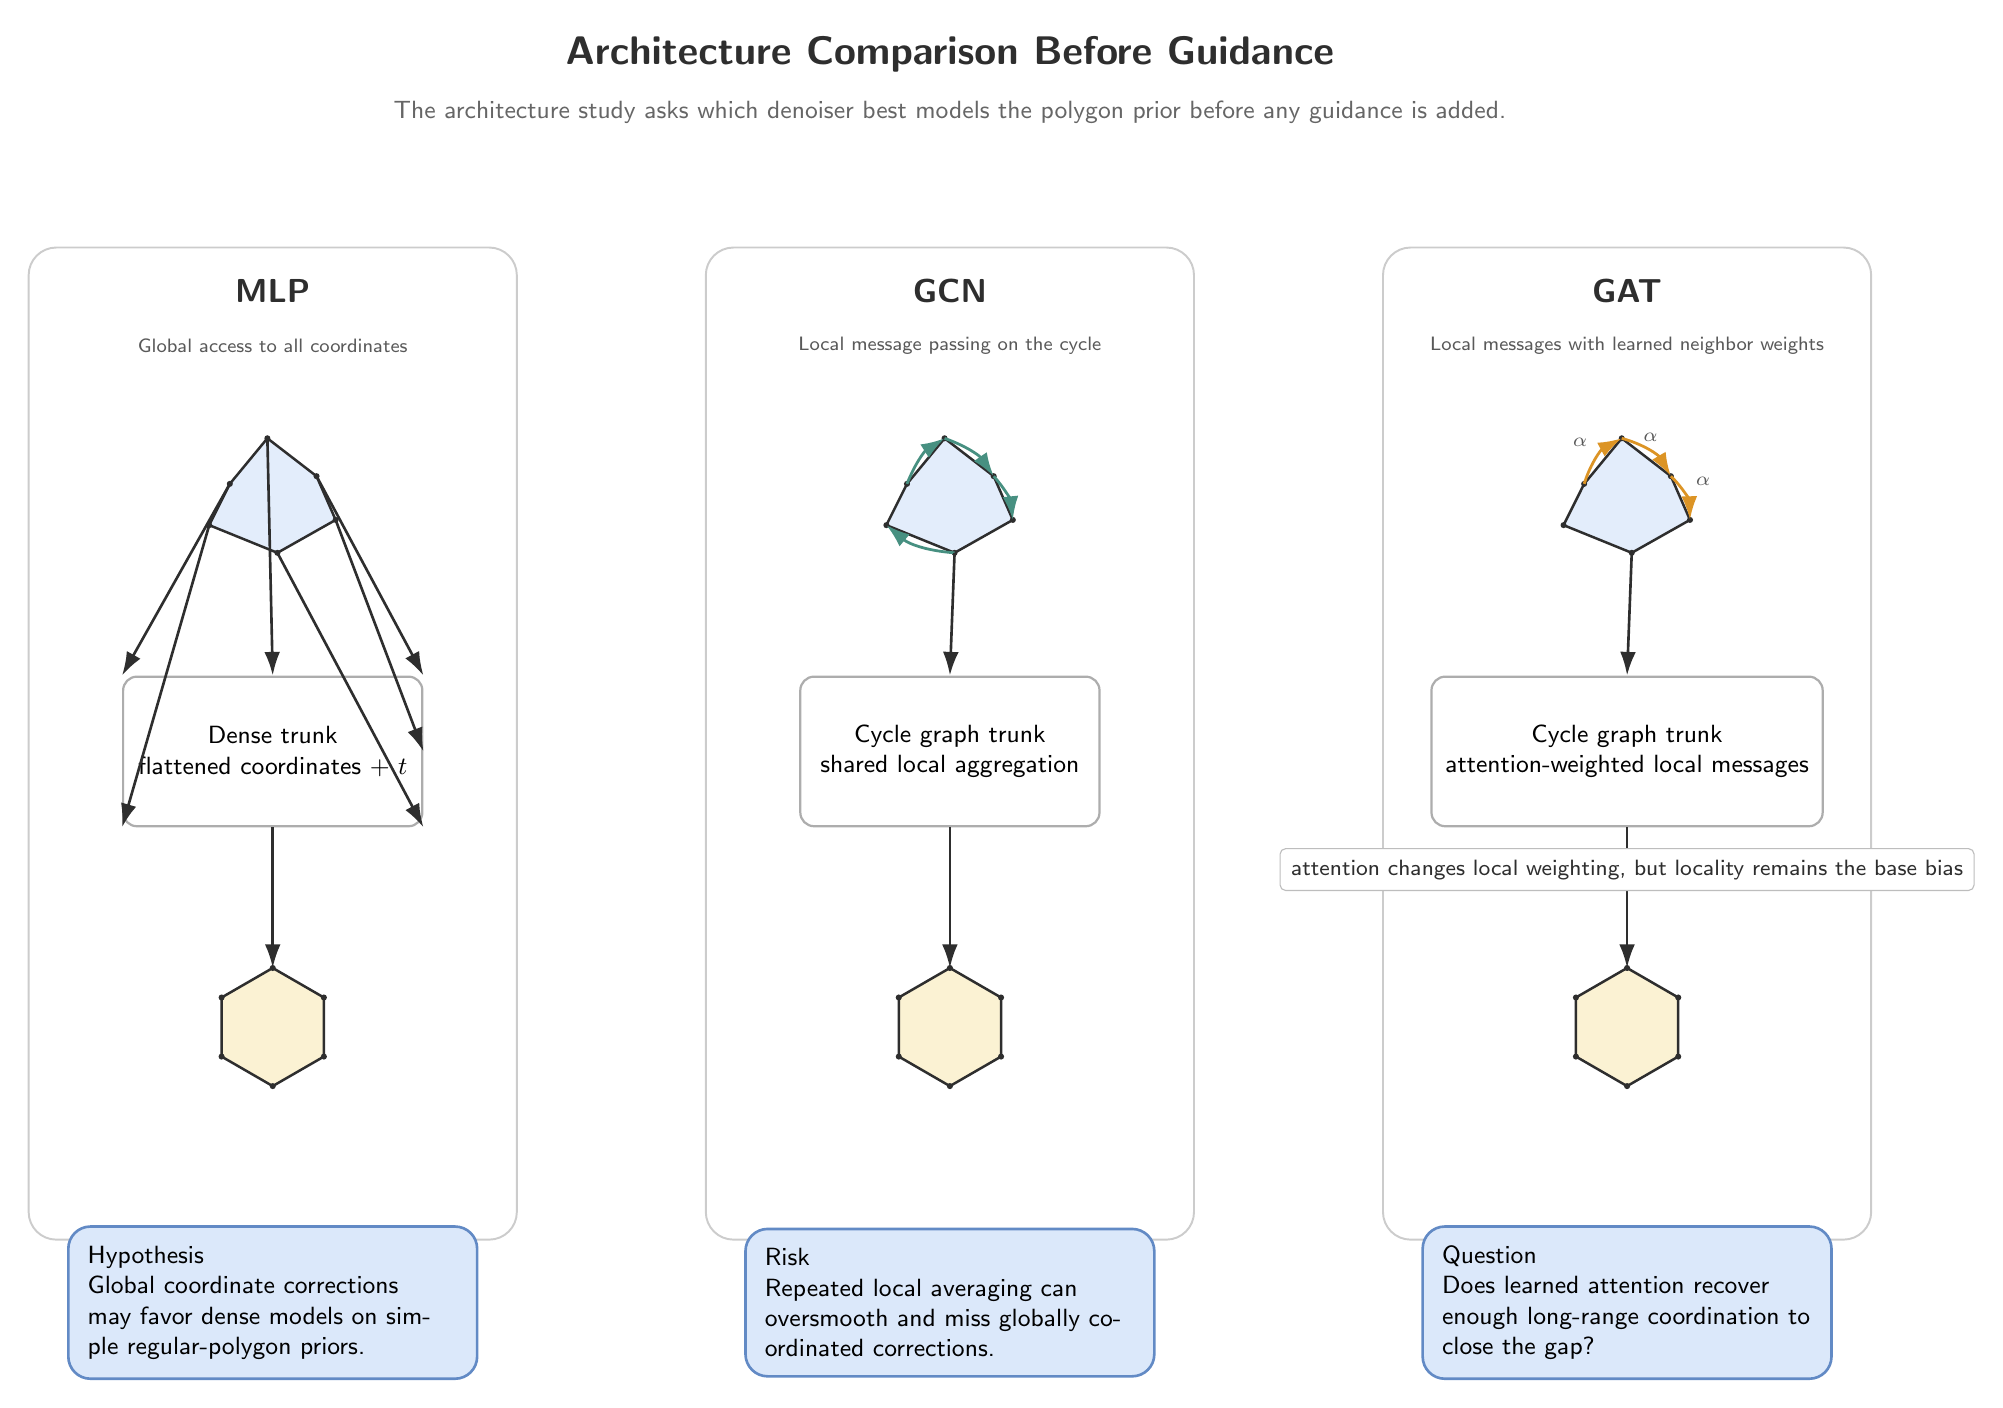
\begin{tikzpicture}[x=1cm,y=1cm]
  \PageTitle{Architecture Comparison Before Guidance}
  \PageSubtitle{The architecture study asks which denoiser best models the polygon prior before any guidance is added.}

  \node[outline, fill=white] (col1) at (4.6,9.7) [minimum width=6.2cm, minimum height=12.6cm] {};
  \node[outline, fill=white] (col2) at (13.2,9.7) [minimum width=6.2cm, minimum height=12.6cm] {};
  \node[outline, fill=white] (col3) at (21.8,9.7) [minimum width=6.2cm, minimum height=12.6cm] {};

  \node[font=\sffamily\bfseries\large, text=ink] at (4.6,15.45) {MLP};
  \node[font=\sffamily\bfseries\large, text=ink] at (13.2,15.45) {GCN};
  \node[font=\sffamily\bfseries\large, text=ink] at (21.8,15.45) {GAT};

  \node[tiny label] at (4.6,14.75) {Global access to all coordinates};
  \node[tiny label] at (13.2,14.75) {Local message passing on the cycle};
  \node[tiny label] at (21.8,14.75) {Local messages with learned neighbor weights};

  \pic (mlpin) at (4.6,12.8) {irregularpoly};
  \pic (gcnin) at (13.2,12.8) {irregularpoly};
  \pic (gatin) at (21.8,12.8) {irregularpoly};

  \node[plainbox, minimum width=3.8cm, minimum height=1.9cm] (mlpblock) at (4.6,9.6) {Dense trunk\\flattened coordinates + $t$};
  \node[plainbox, minimum width=3.8cm, minimum height=1.9cm] (gcnblock) at (13.2,9.6) {Cycle graph trunk\\shared local aggregation};
  \node[plainbox, minimum width=3.8cm, minimum height=1.9cm] (gatblock) at (21.8,9.6) {Cycle graph trunk\\attention-weighted local messages};

  \pic (mlpout) at (4.6,6.1) {hexagon};
  \pic (gcnout) at (13.2,6.1) {hexagon};
  \pic (gatout) at (21.8,6.1) {hexagon};

  \draw[arrow] (mlpin-B) -- (mlpblock.north east);
  \draw[arrow] (mlpin-A) -- (mlpblock.north);
  \draw[arrow] (mlpin-F) -- (mlpblock.north west);
  \draw[arrow] (mlpin-C) -- (mlpblock.east);
  \draw[arrow] (mlpin-D) -- (mlpblock.south east);
  \draw[arrow] (mlpin-E) -- (mlpblock.south west);
  \draw[arrow] (mlpblock.south) -- (mlpout-A);

  \draw[connector, line width=1.0pt, tealStroke, ->] (gcnin-A) to[bend left=18] (gcnin-B);
  \draw[connector, line width=1.0pt, tealStroke, ->] (gcnin-B) to[bend left=18] (gcnin-C);
  \draw[connector, line width=1.0pt, tealStroke, ->] (gcnin-D) to[bend left=18] (gcnin-E);
  \draw[connector, line width=1.0pt, tealStroke, ->] (gcnin-F) to[bend left=18] (gcnin-A);
  \draw[arrow] (gcnin-D) -- (gcnblock.north);
  \draw[arrow] (gcnblock.south) -- (gcnout-A);

  \draw[connector, line width=1.0pt, accentStroke, ->] (gatin-A) to[bend left=22] node[tiny label, above] {$\alpha$} (gatin-B);
  \draw[connector, line width=1.0pt, accentStroke, ->] (gatin-B) to[bend left=22] node[tiny label, above right] {$\alpha$} (gatin-C);
  \draw[connector, line width=1.0pt, accentStroke, ->] (gatin-F) to[bend left=22] node[tiny label, above left] {$\alpha$} (gatin-A);
  \draw[arrow] (gatin-D) -- (gatblock.north);
  \draw[arrow] (gatblock.south) -- (gatout-A);
  \node[note] at (21.8,8.1) {attention changes local weighting, but locality remains the base bias};

  \node[bluebox, text width=4.7cm, minimum height=1.65cm] at (4.6,2.6) {Hypothesis\\Global coordinate corrections may favor dense models on simple regular-polygon priors.};
  \node[bluebox, text width=4.7cm, minimum height=1.65cm] at (13.2,2.6) {Risk\\Repeated local averaging can oversmooth and miss globally coordinated corrections.};
  \node[bluebox, text width=4.7cm, minimum height=1.65cm] at (21.8,2.6) {Question\\Does learned attention recover enough long-range coordination to close the gap?};
\end{tikzpicture}
\end{center}
\newpage

% --------------------------------------------------------------------------
% Figure 4
% --------------------------------------------------------------------------
\begin{center}
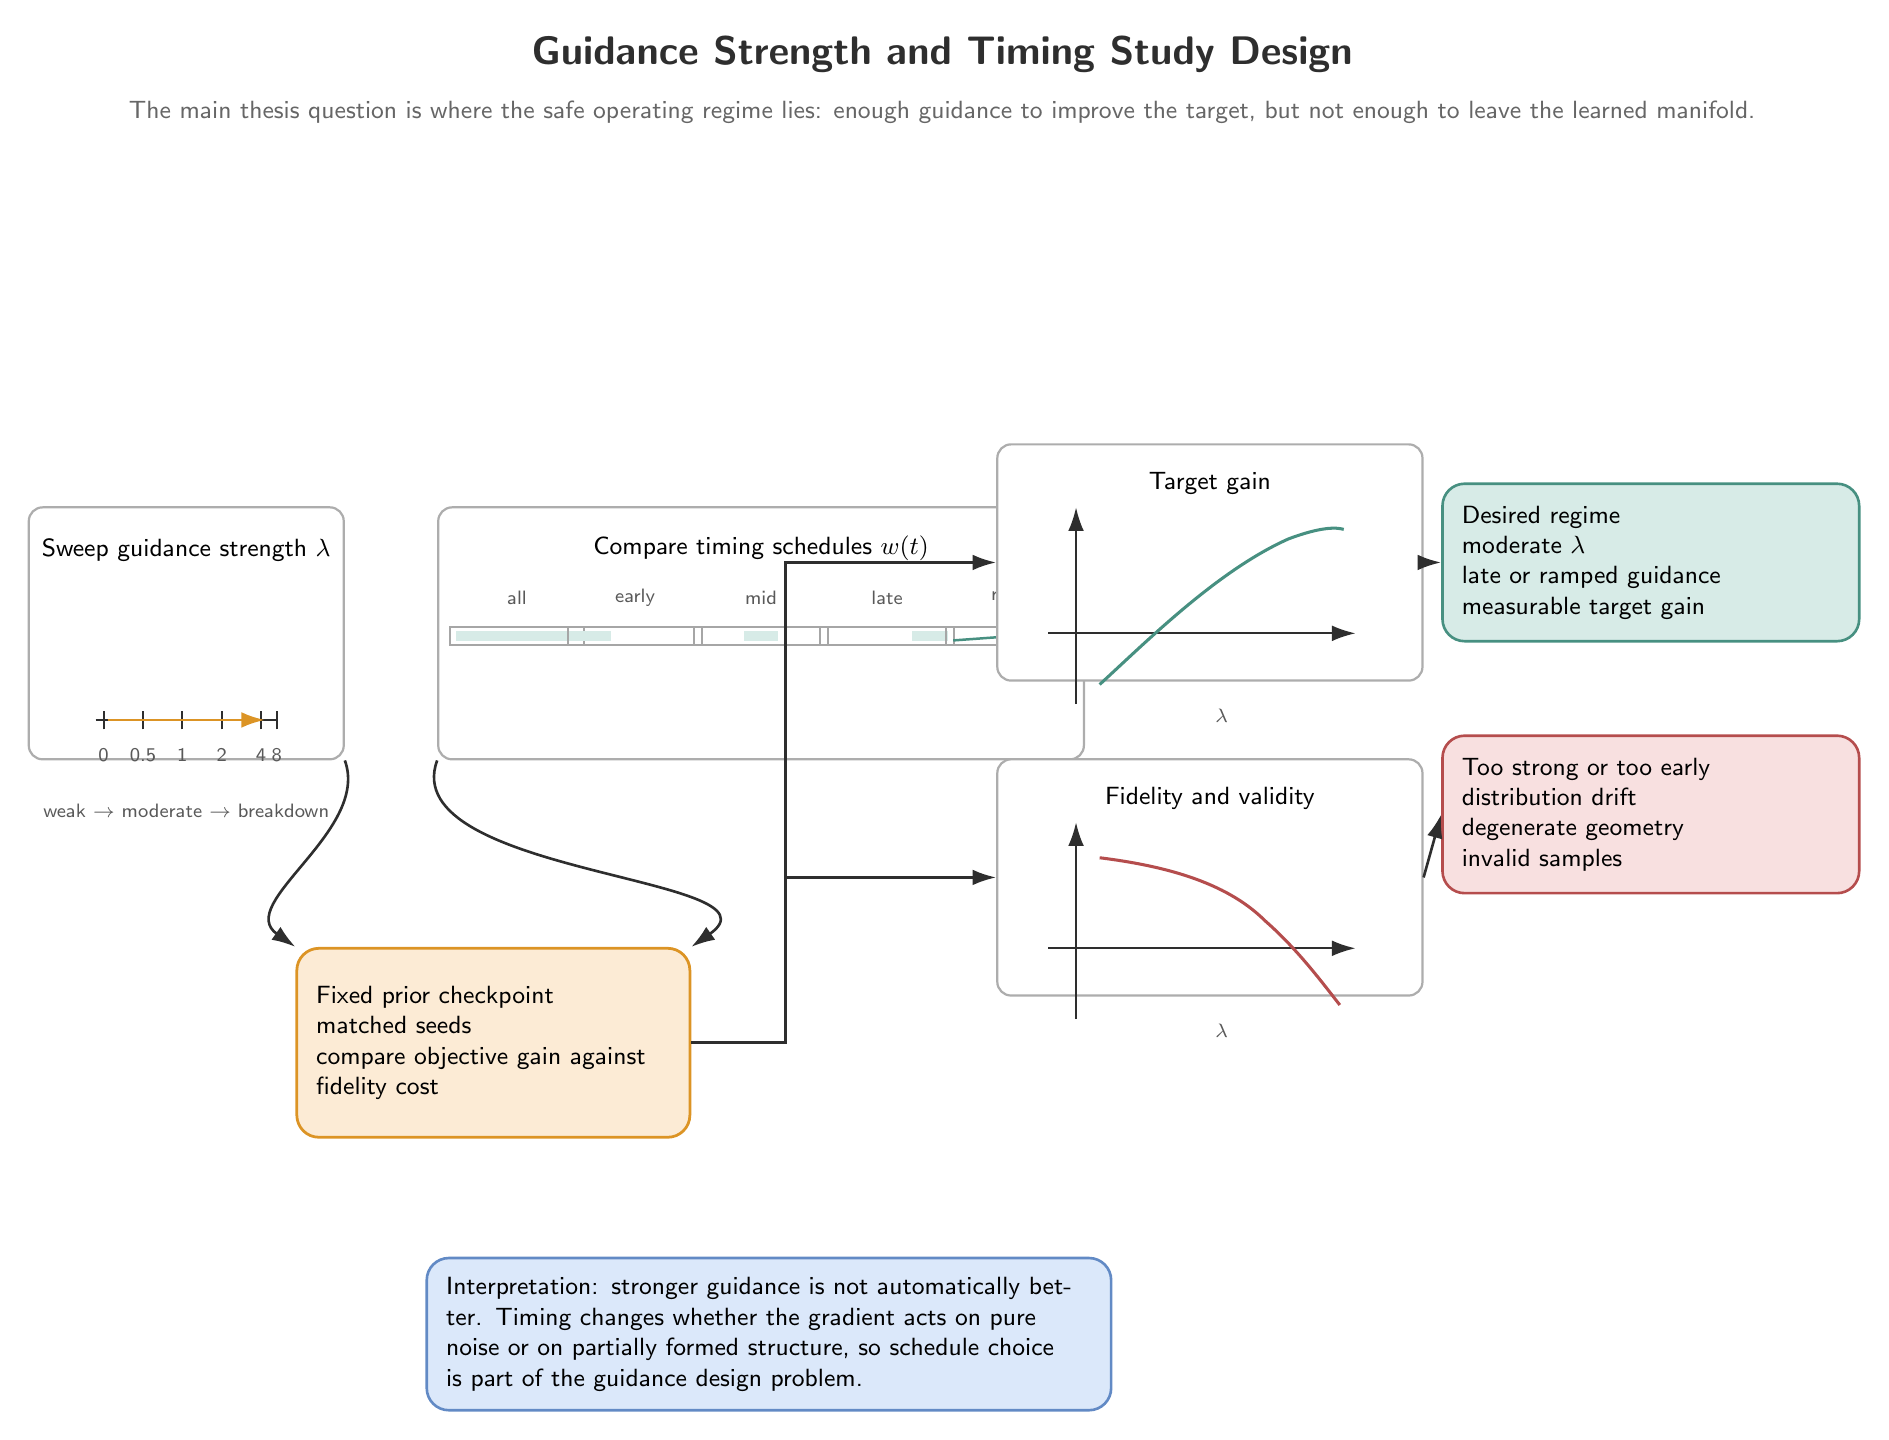
\begin{tikzpicture}[x=1cm,y=1cm]
  \PageTitle{Guidance Strength and Timing Study Design}
  \PageSubtitle{The main thesis question is where the safe operating regime lies: enough guidance to improve the target, but not enough to leave the learned manifold.}

  \node[plainbox, minimum width=4.0cm, minimum height=3.2cm] (lambda) at (3.6,11.1) {};
  \node[font=\sffamily\small] at (3.6,12.15) {Sweep guidance strength $\lambda$};
  \draw[connector, line width=0.9pt] (2.45,10.0) -- (4.75,10.0);
  \foreach \x/\lab in {2.55/0,3.05/0.5,3.55/1,4.05/2,4.55/4,4.75/8}{
    \draw[connector, line width=0.7pt] (\x,9.88) -- (\x,10.12);
    \node[tiny label] at (\x,9.55) {\lab};
  }
  \draw[connector, line width=1.0pt, -{Latex[length=3mm,width=2mm]}, accentStroke] (2.6,10.0) -- (4.6,10.0);
  \node[tiny label] at (3.6,8.85) {weak $\rightarrow$ moderate $\rightarrow$ breakdown};

  \node[plainbox, minimum width=8.2cm, minimum height=3.2cm] (sched) at (10.9,11.1) {};
  \node[font=\sffamily\small] at (10.9,12.18) {Compare timing schedules $w(t)$};

  \node[tiny label] at (7.8,11.55) {all};
  \draw[black!35, line width=0.5pt] (6.95,10.95) rectangle (8.65,11.18);
  \fill[tealFill] (7.02,11.00) rectangle (8.58,11.13);

  \node[tiny label] at (9.3,11.55) {early};
  \draw[black!35, line width=0.5pt] (8.45,10.95) rectangle (10.15,11.18);
  \fill[tealFill] (8.52,11.00) rectangle (9.00,11.13);

  \node[tiny label] at (10.9,11.55) {mid};
  \draw[black!35, line width=0.5pt] (10.05,10.95) rectangle (11.75,11.18);
  \fill[tealFill] (10.68,11.00) rectangle (11.12,11.13);

  \node[tiny label] at (12.5,11.55) {late};
  \draw[black!35, line width=0.5pt] (11.65,10.95) rectangle (13.35,11.18);
  \fill[tealFill] (12.82,11.00) rectangle (13.28,11.13);

  \node[tiny label] at (14.1,11.55) {ramp};
  \draw[black!35, line width=0.5pt] (13.25,10.95) rectangle (14.95,11.18);
  \draw[connector, line width=0.9pt, tealStroke] (13.34,11.01) -- (14.86,11.12);

  \node[accentbox, text width=4.5cm, minimum height=2.4cm] (sampler) at (7.5,5.9) {Fixed prior checkpoint\\matched seeds\\compare objective gain against fidelity cost};
  \draw[arrow] (lambda.south east) to[out=-70,in=145] (sampler.north west);
  \draw[arrow] (sched.south west) to[out=-110,in=35] (sampler.north east);

  \node[plainbox, minimum width=5.4cm, minimum height=3.0cm] (gain) at (16.6,12.0) {};
  \node[font=\sffamily\small] at (16.6,13.0) {Target gain};
  \draw[connector, line width=0.7pt, ->] (14.55,11.1) -- (18.45,11.1);
  \draw[connector, line width=0.7pt, ->] (14.9,10.2) -- (14.9,12.7);
  \draw[connector, line width=1.1pt, tealStroke] (15.2,10.45) .. controls (15.8,11.0) and (16.7,11.9) .. (17.6,12.3) .. controls (18.0,12.45) and (18.2,12.45) .. (18.3,12.42);
  \node[tiny label] at (16.75,10.05) {$\lambda$};

  \node[plainbox, minimum width=5.4cm, minimum height=3.0cm] (fidelity) at (16.6,8.0) {};
  \node[font=\sffamily\small] at (16.6,9.0) {Fidelity and validity};
  \draw[connector, line width=0.7pt, ->] (14.55,7.1) -- (18.45,7.1);
  \draw[connector, line width=0.7pt, ->] (14.9,6.2) -- (14.9,8.7);
  \draw[connector, line width=1.1pt, warnStroke] (15.2,8.25) .. controls (16.0,8.15) and (16.8,7.95) .. (17.3,7.45) .. controls (17.7,7.10) and (18.0,6.70) .. (18.25,6.38);
  \node[tiny label] at (16.75,6.05) {$\lambda$};

  \node[warnbox, text width=4.8cm, minimum height=2.0cm] (failure) at (22.2,8.8) {Too strong or too early\\distribution drift\\degenerate geometry\\invalid samples};
  \node[tealbox, text width=4.8cm, minimum height=2.0cm] (safe) at (22.2,12.0) {Desired regime\\moderate $\lambda$\\late or ramped guidance\\measurable target gain};

  \draw[arrow] (sampler.east) -- ++(1.2,0) |- (gain.west);
  \draw[arrow] (sampler.east) -- ++(1.2,0) |- (fidelity.west);
  \draw[arrow] (gain.east) -- (safe.west);
  \draw[arrow] (fidelity.east) -- (failure.west);

  \node[bluebox, text width=8.2cm, minimum height=1.6cm] at (11.0,2.2) {Interpretation: stronger guidance is not automatically better. Timing changes whether the gradient acts on pure noise or on partially formed structure, so schedule choice is part of the guidance design problem.};
\end{tikzpicture}
\end{center}
\newpage

% --------------------------------------------------------------------------
% Figure 5
% --------------------------------------------------------------------------
\begin{center}
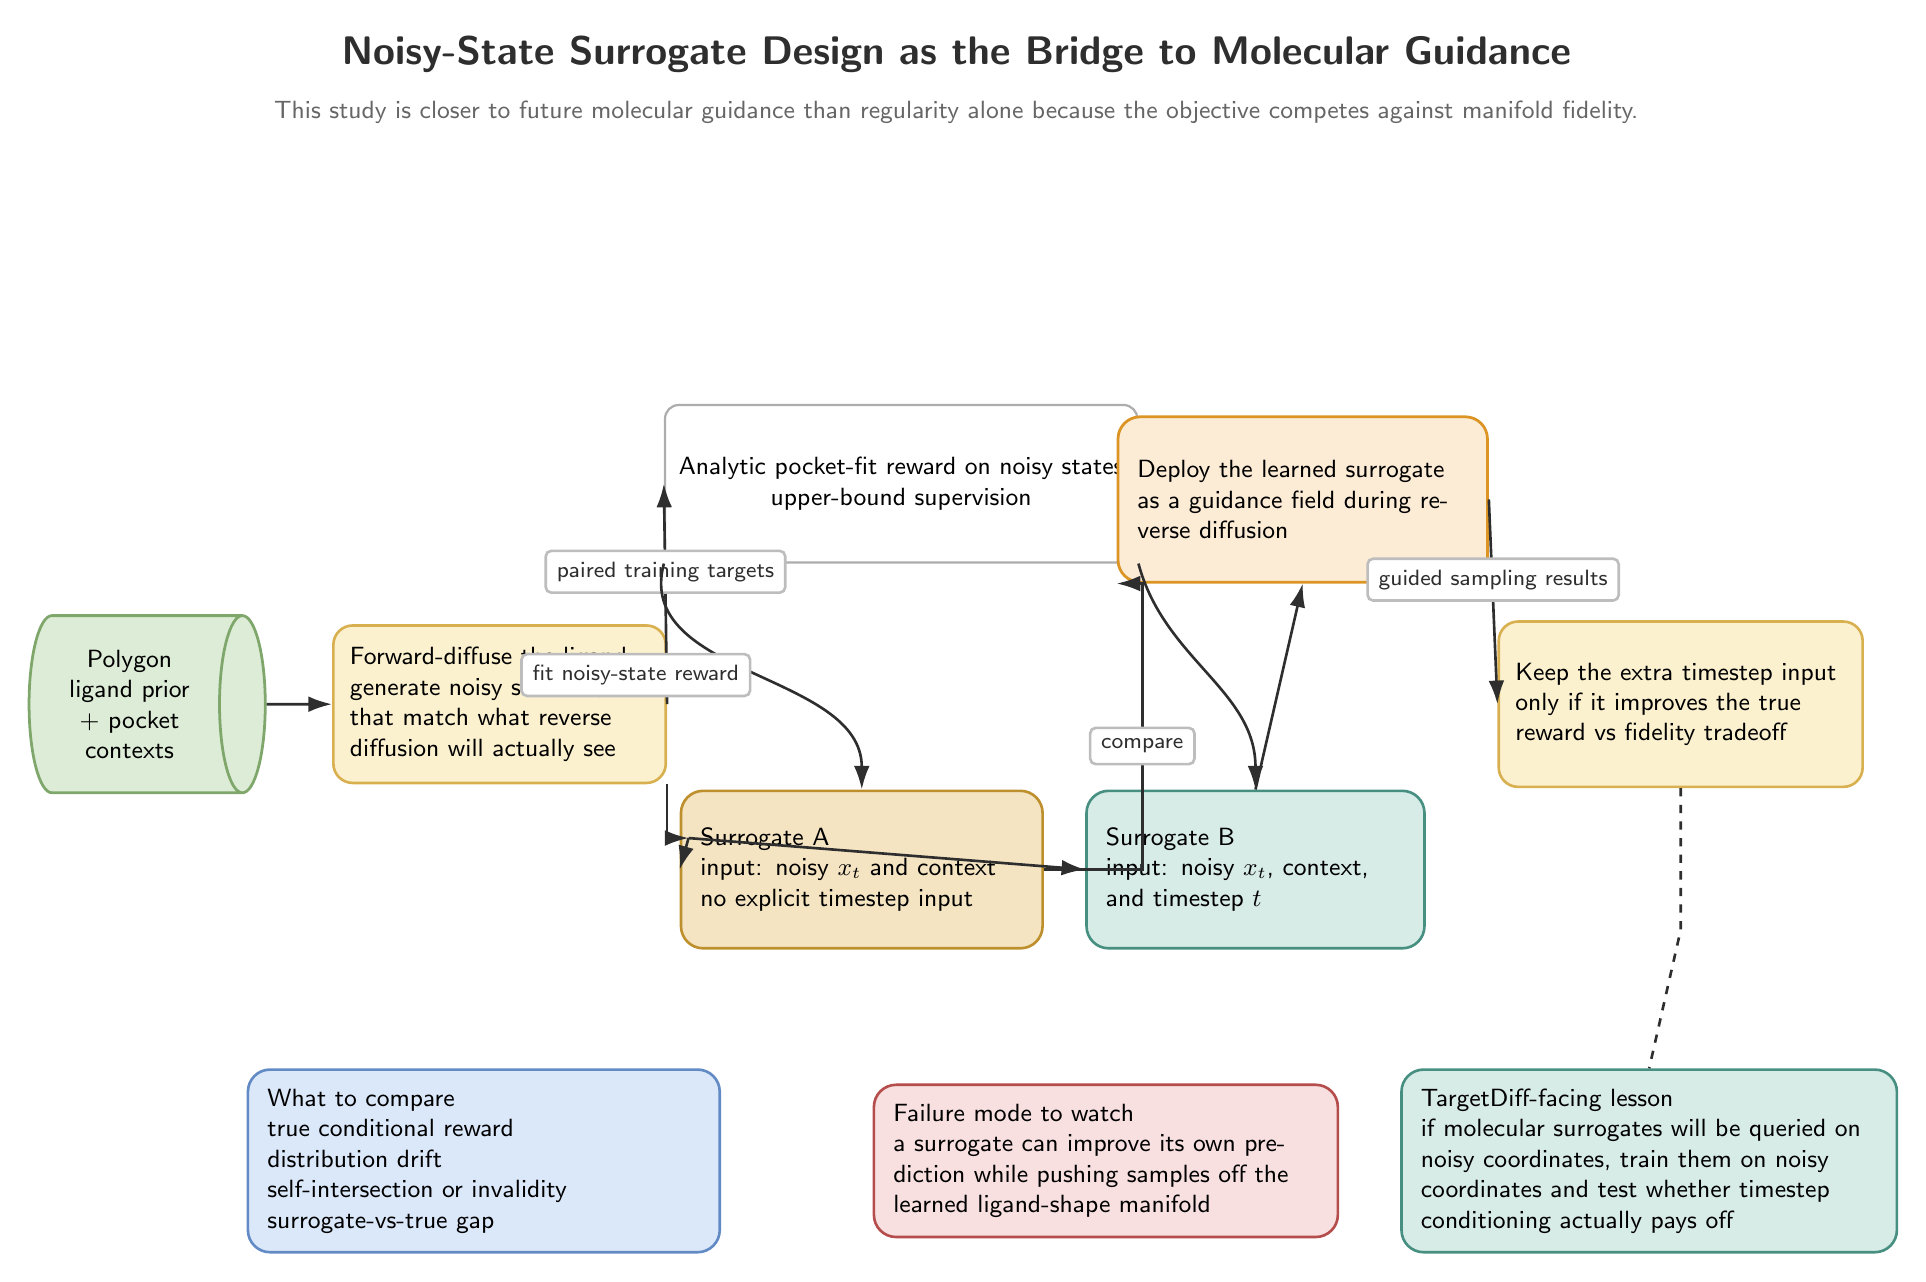
\begin{tikzpicture}[x=1cm,y=1cm]
  \PageTitle{Noisy-State Surrogate Design as the Bridge to Molecular Guidance}
  \PageSubtitle{This study is closer to future molecular guidance than regularity alone because the objective competes against manifold fidelity.}

  \node[databox] (contextdata) at (2.7,10.2) {Polygon\\ligand prior\\+\ pocket\\contexts};
  \node[process, text width=3.8cm, minimum height=2.0cm] (diffuse) at (7.4,10.2) {Forward-diffuse the ligand\\generate noisy states $x_t$ that match what reverse diffusion will actually see};
  \node[plainbox, minimum width=3.7cm, minimum height=2.0cm] (truth) at (12.5,13.0) {Analytic pocket-fit reward on noisy states\\upper-bound supervision};
  \node[amberbox, text width=4.1cm, minimum height=2.0cm] (notime) at (12.0,8.1) {Surrogate A\\input: noisy $x_t$ and context\\no explicit timestep input};
  \node[tealbox, text width=3.8cm, minimum height=2.0cm] (withtime) at (17.0,8.1) {Surrogate B\\input: noisy $x_t$, context, and timestep $t$};
  \node[accentbox, text width=4.2cm, minimum height=2.1cm] (deploy) at (17.6,12.8) {Deploy the learned surrogate as a guidance field during reverse diffusion};
  \node[process, text width=4.2cm, minimum height=2.1cm] (decision) at (22.4,10.2) {Keep the extra timestep input only if it improves the true reward vs fidelity tradeoff};
  \coordinate (branch) at (9.8,8.5);

  \draw[arrow] (contextdata.east) -- (diffuse.west);
  \draw[arrow] (diffuse.east) -- node[note, above] {paired training targets} (truth.west);
  \draw[arrow] (diffuse.south east) |- (branch);
  \draw[arrow] (branch) -- (notime.west);
  \draw[arrow] (branch) -- (withtime.west);
  \draw[arrow] (truth.south west) to[out=-105,in=90] node[note, left] {fit noisy-state reward} (notime.north);
  \draw[arrow] (truth.south east) to[out=-75,in=90] (withtime.north);
  \draw[arrow] (notime.east) -- ++(1.25,0) |- node[note, near start, below] {compare} (deploy.south west);
  \draw[arrow] (withtime.north) -- (deploy.south);
  \draw[arrow] (deploy.east) -- node[note, above] {guided sampling results} (decision.west);

  \node[bluebox, text width=5.5cm, minimum height=1.8cm] (metricbox) at (7.2,4.4) {What to compare\\true conditional reward\\distribution drift\\self-intersection or invalidity\\surrogate-vs-true gap};
  \node[warnbox, text width=5.4cm, minimum height=1.8cm] (warningbox) at (15.1,4.4) {Failure mode to watch\\a surrogate can improve its own prediction while pushing samples off the learned ligand-shape manifold};
  \node[tealbox, text width=5.8cm, minimum height=1.8cm] (bridgebox) at (22.0,4.4) {TargetDiff-facing lesson\\if molecular surrogates will be queried on noisy coordinates, train them on noisy coordinates and test whether timestep conditioning actually pays off};

  \draw[connector, dashed] (decision.south) -- ++(0,-1.8) -- (bridgebox.north);
\end{tikzpicture}
\end{center}
\newpage

% --------------------------------------------------------------------------
% Figure 6
% --------------------------------------------------------------------------
\begin{center}
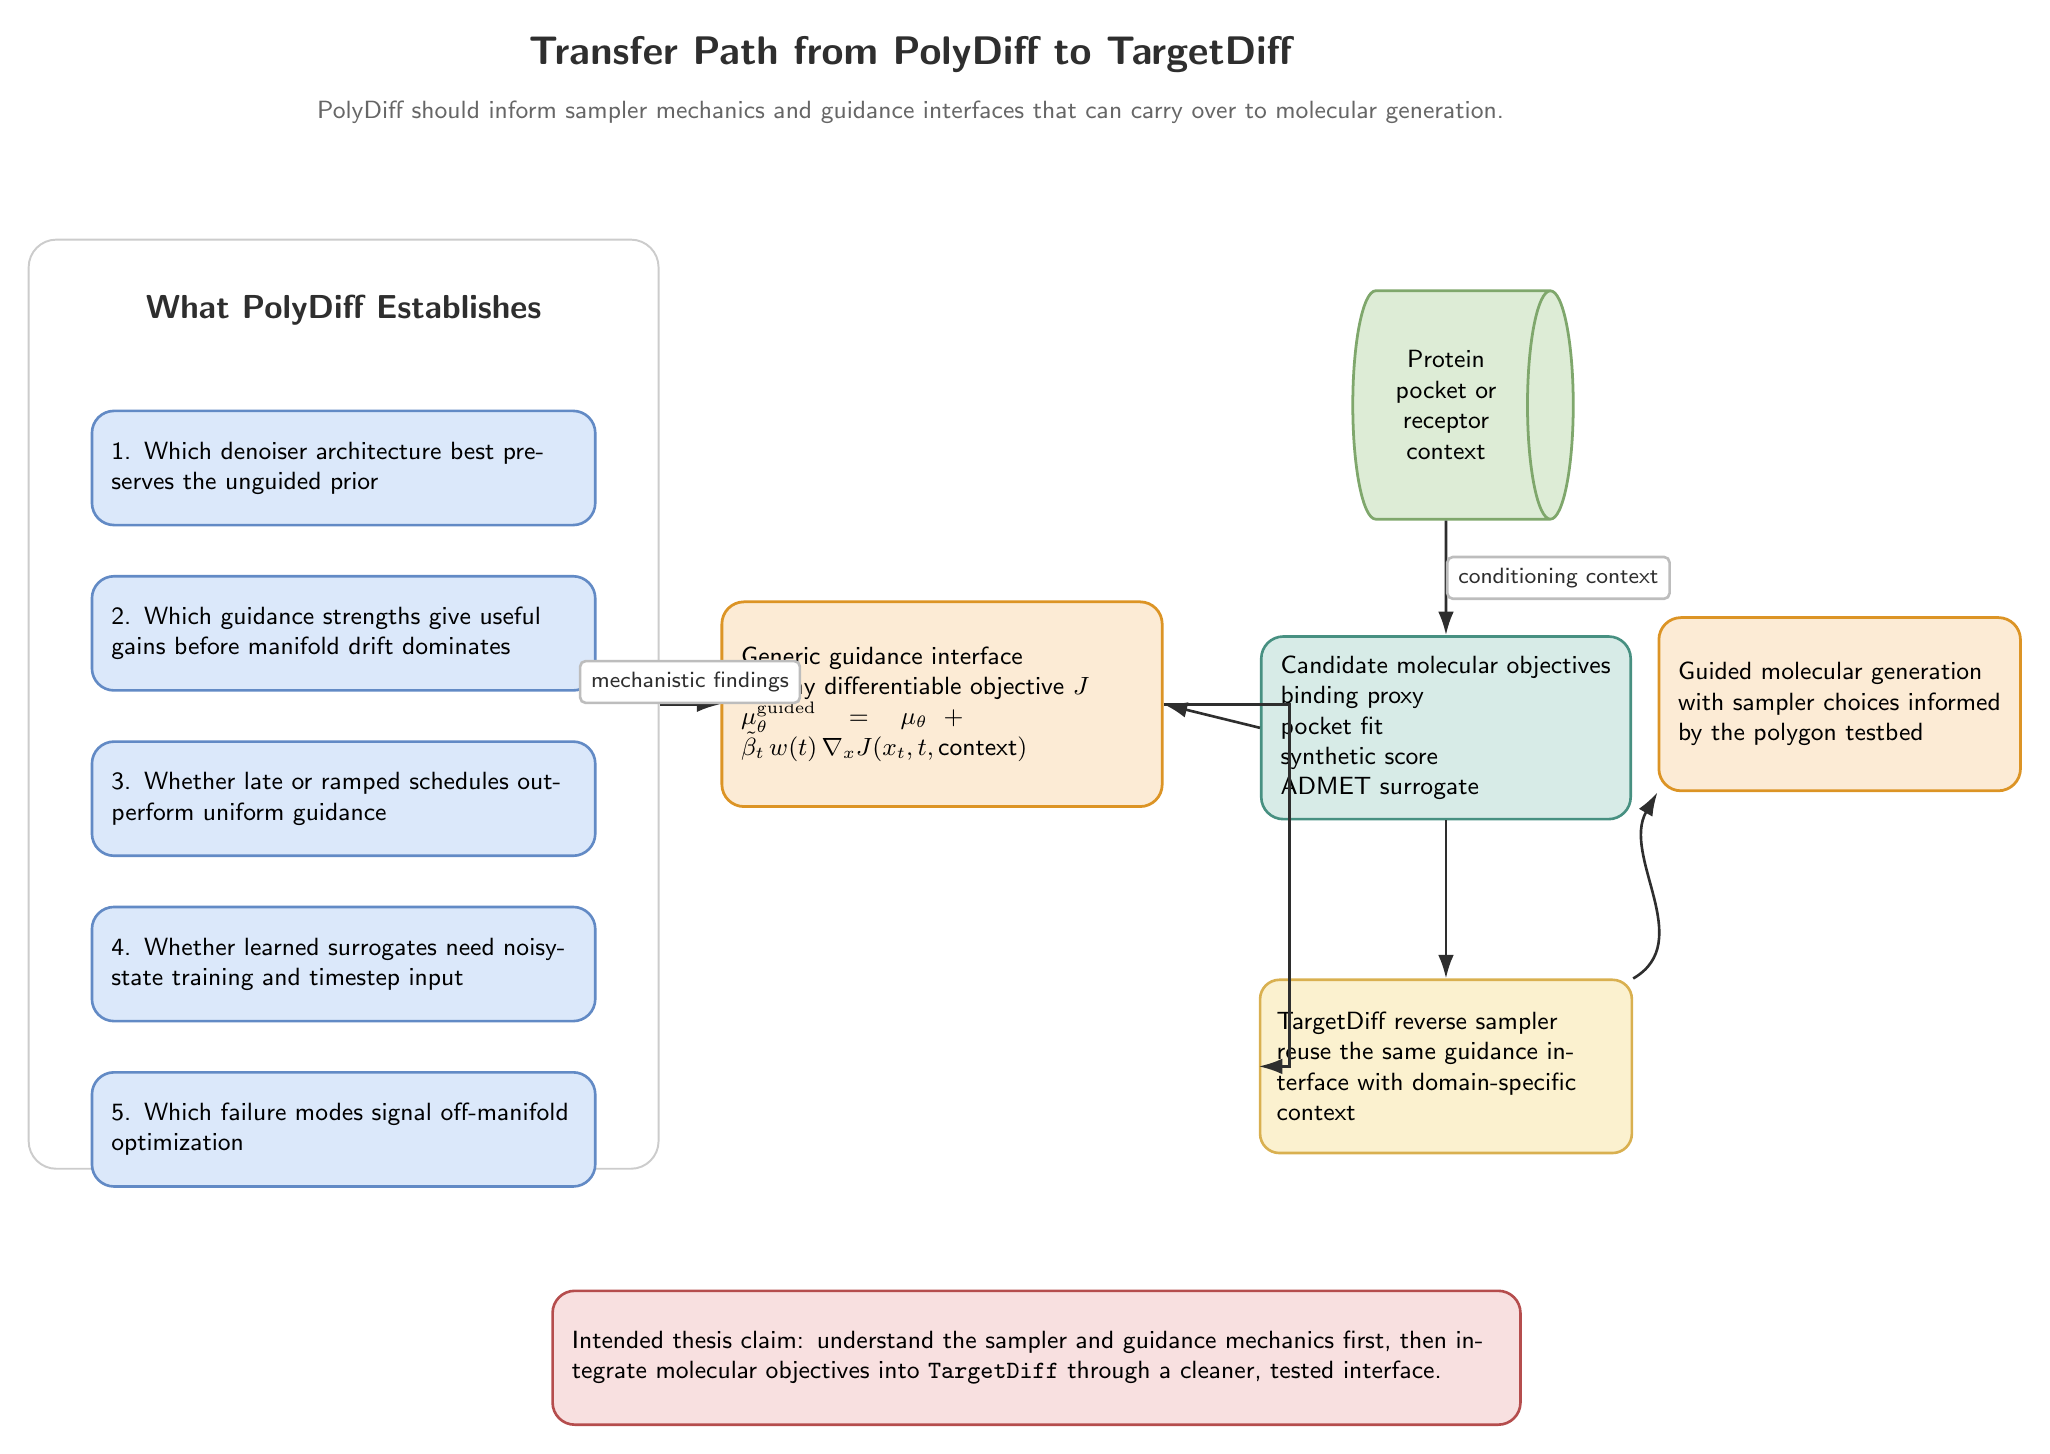
\begin{tikzpicture}[x=1cm,y=1cm]
  \PageTitle{Transfer Path from PolyDiff to TargetDiff}
  \PageSubtitle{PolyDiff should inform sampler mechanics and guidance interfaces that can carry over to molecular generation.}

  \node[outline, fill=white] (leftpanel) at (6.0,10.2) [minimum width=8.0cm, minimum height=11.8cm] {};
  \node[font=\sffamily\bfseries\large, text=ink] at (6.0,15.2) {What PolyDiff Establishes};

  \node[bluebox, text width=5.9cm, minimum height=1.45cm] at (6.0,13.2) {1. Which denoiser architecture best preserves the unguided prior};
  \node[bluebox, text width=5.9cm, minimum height=1.45cm] at (6.0,11.1) {2. Which guidance strengths give useful gains before manifold drift dominates};
  \node[bluebox, text width=5.9cm, minimum height=1.45cm] at (6.0,9.0) {3. Whether late or ramped schedules outperform uniform guidance};
  \node[bluebox, text width=5.9cm, minimum height=1.45cm] at (6.0,6.9) {4. Whether learned surrogates need noisy-state training and timestep input};
  \node[bluebox, text width=5.9cm, minimum height=1.45cm] at (6.0,4.8) {5. Which failure modes signal off-manifold optimization};

  \node[accentbox, text width=5.1cm, minimum height=2.6cm] (interface) at (13.6,10.2) {Generic guidance interface\\for any differentiable objective $J$\\$\mu_\theta^{\mathrm{guided}} = \mu_\theta + \tilde{\beta}_t\,w(t)\,\nabla_x J(x_t,t,\text{context})$};

  \node[databox, minimum width=2.9cm, minimum height=2.8cm] (protein) at (20.0,14.0) {Protein\\pocket or\\receptor\\context};
  \node[tealbox, text width=4.2cm, minimum height=2.1cm] (objectives2) at (20.0,9.9) {Candidate molecular objectives\\binding proxy\\pocket fit\\synthetic score\\ADMET surrogate};
  \node[process, text width=4.3cm, minimum height=2.2cm] (targetsampler) at (20.0,5.6) {TargetDiff reverse sampler\\reuse the same guidance interface with domain-specific context};
  \node[accentbox, text width=4.1cm, minimum height=2.2cm] (outcome2) at (25.0,10.2) {Guided molecular generation\\with sampler choices informed by the polygon testbed};

  \draw[arrow] (leftpanel.east) -- node[note, above] {mechanistic findings} (interface.west);
  \draw[arrow] (protein.south) -- node[note, right] {conditioning context} (objectives2.north);
  \draw[arrow] (objectives2.west) -- (interface.east);
  \draw[arrow] (interface.east) -- ++(1.6,0) |- (targetsampler.west);
  \draw[arrow] (objectives2.south) -- (targetsampler.north);
  \draw[arrow] (targetsampler.north east) to[out=30,in=-120] (outcome2.south west);

  \node[warnbox, text width=11.8cm, minimum height=1.7cm] at (14.8,1.9) {Intended thesis claim: understand the sampler and guidance mechanics first, then integrate molecular objectives into \texttt{TargetDiff} through a cleaner, tested interface.};
\end{tikzpicture}
\end{center}

\end{document}
